\documentclass[12pt]{standalone}
\usepackage{graphicx}
\usepackage[version=4]{mhchem}
%% Color package and configuration.
\usepackage[dvipsnames]{xcolor}
\usepackage{tikz}
\usepackage[per-mode=fraction]{siunitx}
\usepackage{pgfplots}
\usepackage{circuitikz}
\usepackage{amsmath,amssymb,xfrac}

%% Commands package.
\usepackage{etoolbox}

%% Fonts package.
\usepackage[no-math]{fontspec}

%%% Configure pgf and tikz.

\pgfplotsset{
    compat=1.18,
    colormap={quanteem}{rgb255=(18, 45, 141) rgb255=(249, 18, 60)}
}

\usetikzlibrary{arrows.meta}
\definecolor{cyan}{HTML}{5BCEFA}
\definecolor{purple}{HTML}{A30262}
\definecolor{green}{HTML}{006b6b}
\definecolor{Blue}{HTML}{091540}

\definecolor{QuanTEEMRed}{HTML}{F9123C}
\definecolor{QuanTEEMBlue}{HTML}{122D8D}
\definecolor{QuanTEEMOrange}{HTML}{FF6700}

%% Color package and configuration.
\usepackage{xcolor}

\begin{document}

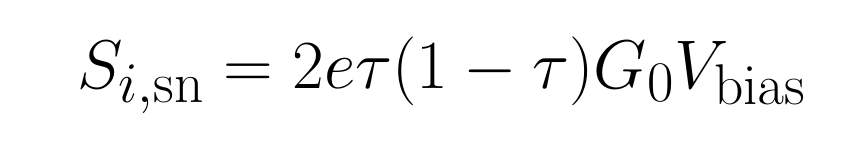
\begin{tikzpicture}

    % \draw [opacity=0] (-5.25, 0) rectangle++ (12.25, -4.75);
    \draw [opacity=0] (-5.25, 0) rectangle++ (10.25, 0.25);

    \node at (0, 0) {
        \Huge \(
            S_{i, \text{sn}} = 2e
            % \left|\langle I\rangle\right| F
            \tau (1-\tau) G_0 V_\text{bias}
        \)
    };

    % \draw [-Latex, thick, opacity=0] (1.44, -0.5)
    % to[in=90, out=270]++ (-4, -2)
    % node[below] {\Huge \(
    %     0
    %     % G_0 V_\text{bias}
    %     % \tau G_0 V_\text{bias}
    %     % \sum_k \tau_k G_0 V_\text{bias}
    % \)};

    % \draw [-Latex, thick, opacity=0] (2.74, -0.5)
    % to[in=90, out=270]++ (2, -2)
    % node[below] {\Huge \(
    %     % 1
    %     % 0
    %     % (1-\tau)
    %     \frac{\sum_k \tau_k (1-\tau_k)}{\sum_k \tau_k}
    % \)};

\end{tikzpicture}
\end{document}
